\documentclass[12pt,a4paper]{article}
\usepackage[utf8]{inputenc}
\usepackage[T1]{fontenc}
\usepackage[utf8]{inputenc}
\usepackage[french]{babel}
\usepackage{graphicx}
\usepackage[T1]{fontenc}
\usepackage{graphicx}





\begin{document}
\begin{figure}

\end{figure}
\section*{Introduction}
  Youtube  est un site web d'hébergement de vidéos et média social sur lequel les utilisateurs ont la possibilité d'envoyer, regarder, 
commenter, évaluer et partager des vidéos en streaming.le machine learning est un domaine d'investigation consacré à la compréhension et 
à la construction de méthodes qui
 «apprennent», c'est-à-dire des méthodes qui exploitent les données pour améliorer les performances sur un ensemble de tâches. Ainsi,Les 
révolutions scientifiques sont toujours inspirées de la nature humaine, qu'elles soient physique ou intellectuelle. Ainsi 
quelle place occupe le Machine Learning dans le système de recommandation de YouTube? Et comment fonctionne le système de recommandation
 de Youtube? Repondre a ces questions fera l'objet de notre étude. 
 
\section{Le Machine Learning dans le système de recommandation}
 Nous pouvons effectuer différentes activités sur YouTube. Alors, Lorsque nous effectuons des recherches sur Youtube, Automatiquement Youtube nous recommande  Recommande des résultats, propose des résultats et nous  suggère. en fonction de notre recherche , Les recommandations sont celles capables de de nous plaire ou de nous apporter satisfaction à une recherche.

 
\section{Approche base sur le contenu}	
 une approche basé sur le contenu consiste a repérer les éléments qui correspondent le mieux avec les préférences de l'utilisateur. Cette technique se focalise sur les caractéristiques des produits afin de recommander aux utilisateurs les produits qui auront de nouvelles propriétés 
similaire avec des produits avec lesquels ils ont déjà interagit; Il s'agit du contenu similaire avec celui que j'ai aimé.


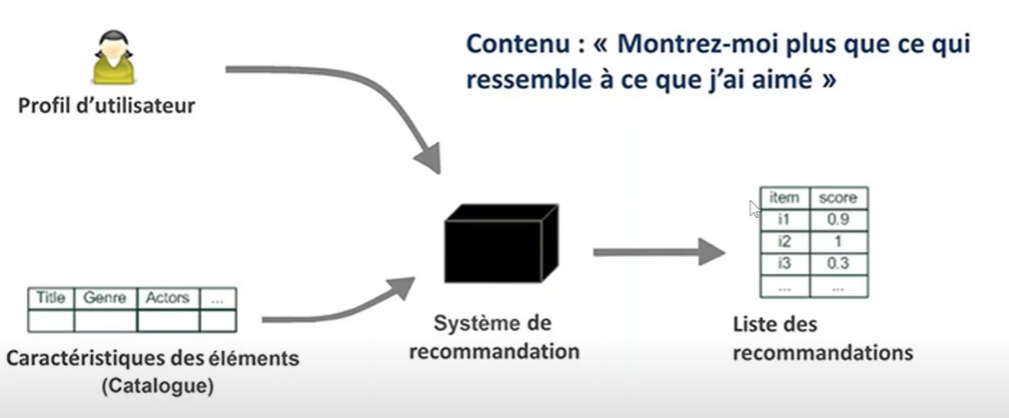
\includegraphics[width=2\linewidth]{Capture 1}





Ici, il cherche à établir des profils descriptifs des utilisateurs puis à comparer ces profils aux données rencontrees pendant leurs navigation. L'ypothese de travail est : "L'utilisateur x aime les items presentant les caracteristiques {c1,...cn}, Nous pouvons lui recommander des items presentants les memes caracteristiques.




\section{Approche basée sur le filtrage collaboratif }	
Une approche basée sur le filtrage collaboratif produisent des recommandations en calculant la similarité entre les préférences d'un utilisateur et d'autres utilisateurs. Cette méthode s'appuie sur l'information relative aux utilisateurs pour calculer la similarité entre deux produits utilisateurs.

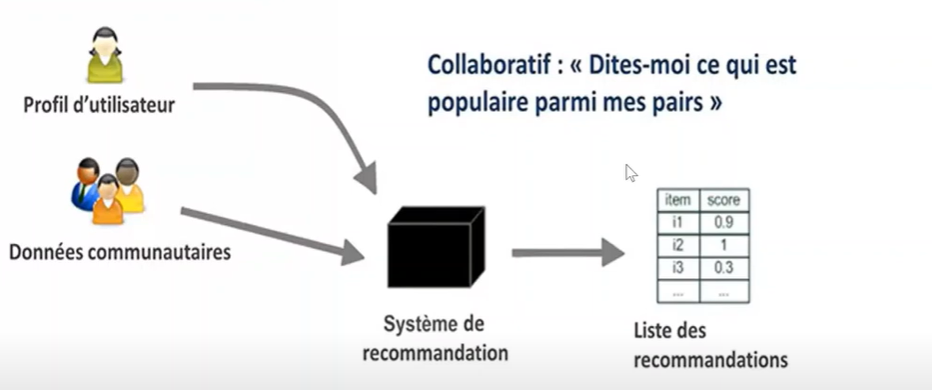
\includegraphics[width=2\linewidth]{Capture2}




 Ici le Systeme de recommandation cherche a croiser les navigations des utilisateurs pour faire profiter les uns des liens entre donnees recoltees sur les autres. La liason entre un item et un utilisateur se fait sur la base de l'hypothese suivante : "les utilisateurs qui ont aimé les memes items que l'utilisateur x aiment aussi ces items la que nous pouvons recommander a x'".
 
 \subsection{Collecte de données}
 Directe : Par l'evalution directe de l'utilisateur. La nous avons une evalution de l'utilisateur des vidéos auxquels il a apporté un avis
 
Indirecte :Donnees obtenues par l'évaluation indirecte de l'utilisateur . Ici le systeme de recommandation observe si l'utilisateur a observe si l'utilisateur a regardé une video entierement,à moitié ou quelques minutes. En fonction de ses differents cricteres on peut collecter les donnees sur une donnees.

\subsection{User-To-User}
Les recommandations sont faites en trouvant des utilisateurs ayant des avis similaire. En exemple nous pouvons ennumerer : "Bidias et Paul aiment tous les deux l'items 2 et n'aime pas l'Iterm 3, il semble qu'ils ont des avis similaire, ce qui suggere qu'en generel Bidias et Paul sont du meme avis. Donc l'Item1 est une bonne recommandation pour Paul
\subsection{Iterm-To-Iterm}
Les recommandations sont faites en trouvant les items qui ont le meme interet par plusieurs utilisateurs. Ricardo et Sandra aime L'Item 1 et L'Item 4. cela suggere qu'en general, les utilisateurs qui aiment l'Item 4 aimerons aussi L'iterms 1.Ainsi ,L'items 1 Pourra etre recommande a Tim. 
\section{Approche hybride}
L'approche hybride utilisent de différents types d'approche de recommandation ou s'appuie sur la leurs logique. Par exemple un tel système peut utiliser a la fois des connaissances extérieures et les caractéristiques des éléments combinant ainsi des approches collaboratives basées sur le contenu.	
\section{Système de recommandation d'après notre recherche}
Ici ,En fonction de notre recherche , YouTube peut nous recommander des vidéos similaire a notre
recherche. Alors ce qui va se passer dans ce cas c'est que l'algorithme va utiliser les différents termes(expressions) de notre recherche et aller
dans la base de données rechercher les éléments similaires. Et lorsque nous Postons une vidéo sous youTube nous mettons les différents mots 
susceptibles de retrouver notre vidéos 

\section{Le système de recommandation en mode }
Le streaming est un type de technologie multimédia qui fournit du contenu vidéo et audio à un appareil connecté à Internet. Cela nous permet d'accéder à du contenu (TV, films, musique, podcasts) à tout moment, sur un ordinateur ou un appareil mobile, sans tenir compte d'une horaire de diffusion. c'est ainsi que de puissant algoritthmes sont definit lors du streaming. Nous avons l'exemple dans       \cite{benbouzid2020cadran} ou l'auteur dit ()


\bibliographystyle{plain}
\bibliography{biblio.bib}
\end{document}
